

\tikzset{every picture/.style={line width=0.75pt}} %set default line width to 0.75pt        

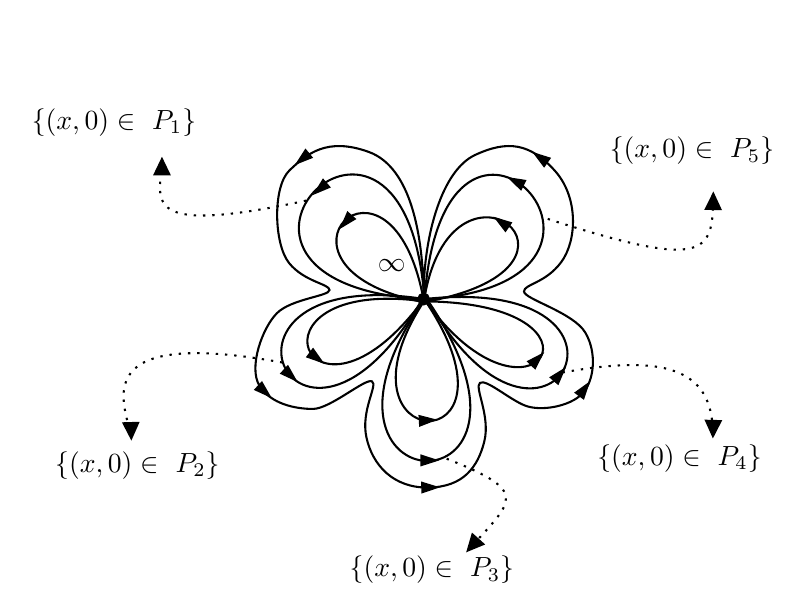
\begin{tikzpicture}[x=0.75pt,y=0.75pt,yscale=-1,xscale=1]
%uncomment if require: \path (0,300); %set diagram left start at 0, and has height of 300

%Curve Lines [id:da30518124245165645] 
\draw    (299.4,141.74) .. controls (244,215.5) and (209.1,128.99) .. (300.34,141.53) ;
%Curve Lines [id:da8950808475599585] 
\draw    (300.34,141.53) .. controls (397.67,142.17) and (352.67,212.5) .. (301.28,141.61) ;
%Shape: Circle [id:dp7083342407214686] 
\draw  [fill={rgb, 255:red, 0; green, 0; blue, 0 }  ,fill opacity=1 ] (297.63,140.42) .. controls (297.63,138.99) and (298.78,137.84) .. (300.21,137.84) .. controls (301.63,137.84) and (302.79,138.99) .. (302.79,140.42) .. controls (302.79,141.84) and (301.63,143) .. (300.21,143) .. controls (298.78,143) and (297.63,141.84) .. (297.63,140.42) -- cycle ;
%Curve Lines [id:da9719941367446978] 
\draw    (298.03,140.42) .. controls (171,131) and (291.07,10.17) .. (300.61,140.42) ;
%Curve Lines [id:da38242804392902285] 
\draw    (300.61,140.42) .. controls (310.2,10.2) and (423.11,131.57) .. (303.19,140.42) ;
%Curve Lines [id:da569057900625008] 
\draw    (300.61,140.42) .. controls (419.97,127.57) and (359.97,243.29) .. (301.82,140.54) ;
%Curve Lines [id:da0472317528556514] 
\draw    (299.4,140.72) .. controls (238.6,245) and (183,122.2) .. (300.61,140.42) ;
%Curve Lines [id:da2970606376255487] 
\draw    (300.21,137.84) .. controls (299.75,109.81) and (294.2,77) .. (273.86,69.57) .. controls (253.51,62.14) and (243.8,70.6) .. (235.57,78.43) .. controls (227.34,86.26) and (228.04,113.98) .. (235.38,123.06) .. controls (242.71,132.14) and (254.88,133.13) .. (254.86,136.07) .. controls (254.84,139.01) and (236.57,140.26) .. (229.57,147.19) .. controls (222.57,154.12) and (215.66,173.26) .. (221.1,182.14) .. controls (226.53,191.03) and (238.57,193.36) .. (246.86,193.36) .. controls (255.14,193.36) and (272.14,178.43) .. (275.29,180.07) .. controls (278.43,181.71) and (269.76,193.98) .. (272.67,207.17) .. controls (275.57,220.36) and (285.51,231.43) .. (302.41,231.24) .. controls (319.32,231.04) and (326.32,221.45) .. (329.43,209.07) .. controls (332.54,196.69) and (324.52,183.02) .. (327.33,180.83) .. controls (330.14,178.64) and (341.46,188.77) .. (349.09,191.74) .. controls (356.71,194.71) and (370.71,192.14) .. (376.57,186.07) .. controls (382.43,180) and (383.86,166.43) .. (378.14,156.64) .. controls (372.43,146.86) and (348.57,140.41) .. (348.57,136.79) .. controls (348.57,133.16) and (358.71,133) .. (366.43,122.71) .. controls (374.14,112.43) and (375,91.29) .. (363.29,78.43) .. controls (351.57,65.57) and (341,63.57) .. (325,71) .. controls (309,78.43) and (300.38,109.69) .. (300.21,137.84) -- cycle ;
%Curve Lines [id:da4196238518994797] 
\draw  [dash pattern={on 0.84pt off 2.51pt}]  (360,101.8) .. controls (436.62,126.5) and (439.3,118.43) .. (439.76,91.59) ;
\draw [shift={(439.8,88.6)}, rotate = 90.78] [fill={rgb, 255:red, 0; green, 0; blue, 0 }  ][line width=0.08]  [draw opacity=0] (8.93,-4.29) -- (0,0) -- (8.93,4.29) -- cycle    ;
%Curve Lines [id:da512673420318001] 
\draw  [dash pattern={on 0.84pt off 2.51pt}]  (311.31,217.34) .. controls (351.12,233.17) and (343.97,236.82) .. (322.4,260.56) ;
\draw [shift={(320.71,262.43)}, rotate = 311.95] [fill={rgb, 255:red, 0; green, 0; blue, 0 }  ][line width=0.08]  [draw opacity=0] (8.93,-4.29) -- (0,0) -- (8.93,4.29) -- cycle    ;
%Curve Lines [id:da8363660989464397] 
\draw  [dash pattern={on 0.84pt off 2.51pt}]  (232.14,171) .. controls (137.89,153.8) and (155.95,190.09) .. (159.02,205.68) ;
\draw [shift={(159.4,208.6)}, rotate = 268.26] [fill={rgb, 255:red, 0; green, 0; blue, 0 }  ][line width=0.08]  [draw opacity=0] (8.93,-4.29) -- (0,0) -- (8.93,4.29) -- cycle    ;
%Curve Lines [id:da1537579559441531] 
\draw  [dash pattern={on 0.84pt off 2.51pt}]  (243.57,93) .. controls (163.77,110.1) and (172.93,93.68) .. (174.05,74.85) ;
\draw [shift={(174.14,71.86)}, rotate = 90] [fill={rgb, 255:red, 0; green, 0; blue, 0 }  ][line width=0.08]  [draw opacity=0] (8.93,-4.29) -- (0,0) -- (8.93,4.29) -- cycle    ;
%Shape: Triangle [id:dp8958619795940812] 
\draw  [fill={rgb, 255:red, 0; green, 0; blue, 0 }  ,fill opacity=1 ] (239.39,74.83) -- (243.32,68.72) -- (246.14,72.16) -- cycle ;
%Shape: Triangle [id:dp7323275141016883] 
\draw  [fill={rgb, 255:red, 0; green, 0; blue, 0 }  ,fill opacity=1 ] (247.99,89.28) -- (251.78,83.09) -- (254.69,86.47) -- cycle ;
%Shape: Triangle [id:dp5439908412868601] 
\draw  [fill={rgb, 255:red, 0; green, 0; blue, 0 }  ,fill opacity=1 ] (260.74,105.52) -- (263.63,98.86) -- (266.98,101.8) -- cycle ;
%Shape: Triangle [id:dp6482573513096812] 
\draw  [fill={rgb, 255:red, 0; green, 0; blue, 0 }  ,fill opacity=1 ] (225.83,187.05) -- (219.23,184.03) -- (222.24,180.74) -- cycle ;
%Shape: Triangle [id:dp3538986571399132] 
\draw  [fill={rgb, 255:red, 0; green, 0; blue, 0 }  ,fill opacity=1 ] (238.31,179.28) -- (231.73,176.21) -- (234.76,172.95) -- cycle ;
%Shape: Triangle [id:dp3410795032956404] 
\draw  [fill={rgb, 255:red, 0; green, 0; blue, 0 }  ,fill opacity=1 ] (251.11,170.61) -- (244.26,168.23) -- (246.94,164.67) -- cycle ;
%Shape: Triangle [id:dp4803111514559295] 
\draw  [fill={rgb, 255:red, 0; green, 0; blue, 0 }  ,fill opacity=1 ] (379.46,181.28) -- (377.17,188.17) -- (373.57,185.53) -- cycle ;
%Shape: Triangle [id:dp3708997709224997] 
\draw  [fill={rgb, 255:red, 0; green, 0; blue, 0 }  ,fill opacity=1 ] (367.75,174.42) -- (364.93,181.11) -- (361.55,178.2) -- cycle ;
%Shape: Triangle [id:dp975132604650822] 
\draw  [fill={rgb, 255:red, 0; green, 0; blue, 0 }  ,fill opacity=1 ] (357.14,167.17) -- (353.87,173.65) -- (350.7,170.52) -- cycle ;
%Shape: Triangle [id:dp41553716907224714] 
\draw  [fill={rgb, 255:red, 0; green, 0; blue, 0 }  ,fill opacity=1 ] (335.21,101.69) -- (342.16,103.78) -- (339.62,107.45) -- cycle ;
%Shape: Triangle [id:dp7180277186575779] 
\draw  [fill={rgb, 255:red, 0; green, 0; blue, 0 }  ,fill opacity=1 ] (341.89,82.35) -- (349.06,83.47) -- (347.06,87.45) -- cycle ;
%Shape: Triangle [id:dp33809986896433] 
\draw  [fill={rgb, 255:red, 0; green, 0; blue, 0 }  ,fill opacity=1 ] (353.9,70.48) -- (360.83,72.65) -- (358.26,76.29) -- cycle ;
%Curve Lines [id:da32436656754150617] 
\draw    (301.82,140.54) .. controls (374.2,245.8) and (229.4,243) .. (300.61,140.42) ;
%Curve Lines [id:da8523403673333396] 
\draw    (298.34,141.53) .. controls (215,124.5) and (284.67,54.83) .. (300.34,141.53) ;
%Curve Lines [id:da3938486210267571] 
\draw    (300.34,141.53) .. controls (313,59.83) and (394.67,124.17) .. (302.34,141.53) ;
%Curve Lines [id:da34419357175849075] 
\draw    (301.28,141.61) .. controls (353.67,220.5) and (251.67,216.17) .. (300.34,141.53) ;
%Curve Lines [id:da15164910719694302] 
\draw  [dash pattern={on 0.84pt off 2.51pt}]  (367.14,175.8) .. controls (416.34,166.99) and (439.05,173.71) .. (439.59,204.63) ;
\draw [shift={(439.57,207.57)}, rotate = 271.47] [fill={rgb, 255:red, 0; green, 0; blue, 0 }  ][line width=0.08]  [draw opacity=0] (8.93,-4.29) -- (0,0) -- (8.93,4.29) -- cycle    ;
%Shape: Triangle [id:dp881720647037963] 
\draw  [fill={rgb, 255:red, 0; green, 0; blue, 0 }  ,fill opacity=1 ] (306.11,218.16) -- (299.2,220.38) -- (299.2,215.92) -- cycle ;
%Shape: Triangle [id:dp30862525793679474] 
\draw  [fill={rgb, 255:red, 0; green, 0; blue, 0 }  ,fill opacity=1 ] (306.47,231.14) -- (299.59,233.46) -- (299.54,229) -- cycle ;
%Shape: Triangle [id:dp6612684939262838] 
\draw  [fill={rgb, 255:red, 0; green, 0; blue, 0 }  ,fill opacity=1 ] (305.28,198.67) -- (298.52,201.3) -- (298.25,196.86) -- cycle ;

% Text Node
\draw (276.69,119.97) node [anchor=north west][inner sep=0.75pt]    {$\infty $};
% Text Node
\draw (109.94,47.09) node [anchor=north west][inner sep=0.75pt]    {$\{( x,0) \in \ P_{1}\}$};
% Text Node
\draw (388.4,60.92) node [anchor=north west][inner sep=0.75pt]    {$\{( x,0) \in \ P_{5}\}$};
% Text Node
\draw (121.2,212.4) node [anchor=north west][inner sep=0.75pt]    {$\{( x,0) \in \ P_{2}\}$};
% Text Node
\draw (263.09,262.8) node [anchor=north west][inner sep=0.75pt]    {$\{( x,0) \in \ P_{3}\}$};
% Text Node
\draw (382.4,209.2) node [anchor=north west][inner sep=0.75pt]    {$\{( x,0) \in \ P_{4}\}$};


\end{tikzpicture}